%本章探讨成品需求相关性对改进效果的影响

\chapter{需求相关性对改进效果的影响}

在之前的讨论中,我们总是假设成品的需求分布是相互独立的。事实上,现实中的两种相似成品的需求往往存在一些相关性。本章将讨论成品需求之间的相关性对改进方案的效果的影响。






\section{需求服从二维正态分布的情况}

为了构造相关系数为$\rho$的两个正态分布的需求变量,我们假设两种颜色的成品需求$(D_1,D_2)$服从二维正态分布$N(\mu_1,\mu_2,\sigma_1^2,\sigma_2^2,\rho)$,则它们的联合分布为
\begin{equation}
f(x_1,x_2) = \frac{1}{2\pi\sigma_1\sigma_2\sqrt{1-\rho^2}}e^{-\frac{1}{2(1-\rho^2)}\left[\frac{(x_1-\mu_1)^2}{\sigma_1^2}+\frac{(x_2-\mu_2)^2}{\sigma_2^2}-\frac{2\rho(x_1-\mu_1)(x_2-\mu_2)}{\sigma_1\sigma_2}\right]}
\label{eq:二维正态分布概率密度}
\end{equation}
对$x_2$积分,可以得到$D_1$的边缘分布
\begin{equation}
f_1(x_1) = \int_{-\infty}^{+\infty}\frac{1}{2\pi\sigma_1\sigma_2\sqrt{1-\rho^2}}e^{-\frac{1}{2(1-\rho^2)}\left[\frac{(x_1-\mu_1)^2}{\sigma_1^2}+\frac{(x_2-\mu_2)^2}{\sigma_2^2}-\frac{2\rho(x_1-\mu_1)(x_2-\mu_2)}{\sigma_1\sigma_2}\right]}\dif x_2
\label{eq:二维边缘分布推导}
\end{equation}
令
\[
A = \frac{1}{\sqrt{2\pi}\sigma_1}e^{-\frac{(x_1-\mu_1)^2}{2\sigma_1^2}}
\]
则公式\ref{eq:二维边缘分布推导}可变形为
\begin{equation}
f_1(x_1) = A\int_{-\infty}^{+\infty}\frac{1}{\sqrt{2\pi(1-\rho^2)}\sigma_2}e^{-\frac{1}{2}\left[\frac{\sigma_1(x_2-\mu_2)-\rho\sigma_2(x_1-\mu_1)}{\sqrt{1-\rho^2}\sigma_1\sigma_2}\right]^2}\dif x_2
\label{eq:二维边缘分布变形}
\end{equation}
再令
\[
t = \frac{\sigma_1(x_2-\mu_2)-\rho\sigma_2(x_1-\mu_1)}{\sqrt{1-\rho^2}\sigma_1\sigma_2}
\]
则公式\ref{eq:二维边缘分布变形}可变形为
\begin{equation}
f_1(x_1) = A\int_{-\infty}^{+\infty}\frac{1}{\sqrt{2\pi}}e^{-\frac{t^2}{2}}\dif t
\label{eq:二维边缘分布变形2}
\end{equation}
公式\ref{eq:二维边缘分布变形2}的有半部分是标准正态分布的累积概率,总累积概率应为1,即
\[
\int_{-\infty}^{+\infty}\frac{1}{\sqrt{2\pi}}e^{-\frac{t^2}{2}}\dif t = 1
\]
因此得到$f_1(x_1)=A$,即
\begin{equation}
f_1(x_1) = \frac{1}{\sqrt{2\pi}\sigma_1}e^{-\frac{(x_1-\mu_1)^2}{2\sigma_1^2}}
\label{eq:二维边缘分布1}
\end{equation}
同理有
\begin{equation}
f_2(x_2) = \frac{1}{\sqrt{2\pi}\sigma_2}e^{-\frac{(x_2-\mu_2)^2}{2\sigma_2^2}}
\label{eq:二维边缘分布2}
\end{equation}

公式\ref{eq:二维边缘分布1}和\ref{eq:二维边缘分布2}表明,当需求$D_1$、$D_2$服从二维正态分布$N(\mu_1,\mu_2,\sigma_1^2,\sigma_2^2,\rho)$时,它们分别服从一维正态分布$N(\mu_1,\sigma_1^2)$和$N(\mu_2,\sigma_2^2)$。下面证明,正态分布的两个变量$D_1$、$D_2$之间的相关系数为$\rho$。

由相关系数的定义可知
\begin{align}
\operatorname{Corr}(D_1,D_2) &= \int_{-\infty}^{+\infty}\int_{-\infty}^{+\infty}\frac{(x_1-\mu_1)(x_2-\mu_2)}{\sigma_1\sigma_2}f(x_1,x_2)\dif x_1\dif x_2 \notag\\
&= \int_{-\infty}^{+\infty}\frac{x_2-\mu_2}{\sigma_2}\int_{-\infty}^{+\infty}\frac{x_1-\mu_1}{\sigma_1}f(x_1,x_2)\dif x_1\dif x_2
\label{eq:相关系数定义}
\end{align}
与公式\ref{eq:二维边缘分布变形}类似,令
\[
t = \frac{\sigma_2(x_1-\mu_1)-\rho\sigma_1(x_2-\mu_2)}{\sqrt{1-\rho^2}\sigma_1\sigma_2}
\]
则公式\ref{eq:相关系数定义}变形为
\begin{equation}
\operatorname{Corr}(D_1,D_2) = \int_{-\infty}^{+\infty}\frac{x_2-\mu_2}{\sigma_2}\int_{-\infty}^{+\infty}\frac{e^{-\frac{(x_2-\mu_2)^2}{2\sigma_2^2}}}{2\pi\sigma_2}\left(t\sqrt{1-\rho^2}+\frac{\rho(x_2-\mu_2)}{\sigma_2}\right)e^{-\frac{t^2}{2}}\dif t\dif x_2
\label{eq:相关系数变形}
\end{equation}
易知
\[
\int_{-\infty}^{+\infty}te^{-\frac{t^2}{2}} = 0
\]
且
\[
\int_{-\infty}^{+\infty}e^{-\frac{t^2}{2}} = \sqrt{2\pi}
\]
因此公式\ref{eq:相关系数变形}可得
\begin{align}
\operatorname{Corr}(D_1,D_2) &= \int_{-\infty}^{+\infty}\frac{x_2-\mu_2}{\sigma_2}\left[\frac{\rho(x_2-\mu_2)}{\sqrt{2\pi}\sigma_2^2}\right]\dif x_2 \notag\\
&= \frac{\rho}{\sqrt{2\pi}}\int_{-\infty}^{+\infty}\left(\frac{x_2-\mu_2}{\sigma_2}\right)^2e^{-\frac{1}{2}\left(\frac{x_2-\mu_2}{\sigma_2}\right)^2}\dif \left(\frac{x_2-\mu_2}{\sigma_2}\right)
\label{eq:相关系数变形2}
\end{align}
令
\[
w = \frac{x_2-\mu_2}{\sigma_2}
\]
则公式\ref{eq:相关系数变形2}可变形为
\begin{align}
\operatorname{Corr}(D_1,D_2) &= \frac{\rho}{\sqrt{2\pi}}\int_{-\infty}^{+\infty}w^2e^{-\frac{w^2}{2}}\dif w \notag\\
&= -\frac{\rho}{\sqrt{2\pi}}\int_{-\infty}^{+\infty}w\dif \left(e^{-\frac{w^2}{2}}\right) \notag\\
&= -\frac{\rho}{\sqrt{2\pi}}\left[\left.we^{-\frac{w^2}{2}}\right|_{-\infty}^{+\infty}-\int_{-\infty}^{+\infty}e^{-\frac{w^2}{2}}\dif w\right] \notag\\
&= -\frac{\rho}{\sqrt{2\pi}}\left(0-\sqrt{2\pi}\right) \notag\\
&= \rho
\label{eq:相关系数结果}
\end{align}

至此,我们已构造出两个相关性为$\rho$的需求变量$D_1$和$D_2$,它们各自服从正态分布$N(\mu_1,\sigma_1^2)$和$N(\mu_2,\sigma_2^2)$,并且知道它们的联合分布服从二维正态分布$N(\mu_1,\mu_2,\sigma_1^2,\sigma_2^2,\rho)$。

设企业的服务水平为$\eta$,对应的标准正态分布分位数为$z_\eta$。则两种颜色的成品需要保留的库存$\xi_1$、$\xi_2$分别为
\begin{align}
\xi_1 = \mu_1 + z_\eta\sigma_1 \label{eq:成品库存1_相关性}\\
\xi_2 = \mu_2 + z_\eta\sigma_2 \label{eq:成品库存2_相关性}
\end{align}

现在假设我们按照改进策略,取消两种颜色的成品库存,改为保留未喷涂的在制品库存。忽略供货提前期等变化的影响。企业的服务水平仍然为$\eta$。为了满足该服务水平,所需的在制品库存为$\xi$。此时的在制品库存需要同时应对两种颜色的成品需求,因此,对未喷涂的在制品需求为$D=D_1+D_2$。设$D$、$D_2$的联合分布为$g(y_1,y_2)$。由$y_1=x_1+x_2,y_2=x_2$得$x_1=y_1-y_2,x_2=y_2$。因此,雅可比矩阵为
\[
J = \begin{bmatrix}
\frac{\partial x_1}{\partial y_1} & \frac{\partial x_1}{\partial y_2} \\
\frac{\partial x_2}{\partial y_1} & \frac{\partial x_2}{\partial y_2}
\end{bmatrix} = \begin{bmatrix}
1 & -1 \\
0 & 1
\end{bmatrix}
\]
由此可得$g(y_1,y_2)$的概率分布为
\begin{align}
g(y_1,y_2) &= f(x_1,x_2)\cdot\left|J\right| \notag\\
&= f(y_1-y_2,y_2)\cdot
\begin{vmatrix}
1 & -1 \\
0 & 1
\end{vmatrix} \notag\\
&= \frac{1}{2\pi\sigma_1\sigma_2\sqrt{1-\rho^2}}e^{-\frac{1}{2(1-\rho^2)}\left[\frac{(y_1-y_2-\mu_1)^2}{\sigma_1^2}+\frac{(y_2-\mu_2)^2}{\sigma_2^2}-\frac{2\rho(y_1-y_2-\mu_1)(y_2-\mu_2)}{\sigma_1\sigma_2}\right]}
\label{eq:新联合分布_二维正态}
\end{align}
$g(y_1,y_2)$的边缘分布$h(y_1)$即是在制品需求$D$的概率分布。对$y_2$积分可得
\begin{equation}
h(y_1) = \int_{-\infty}^{+\infty}\frac{1}{2\pi\sigma_1\sigma_2\sqrt{1-\rho^2}}e^{-\frac{1}{2(1-\rho^2)}\left[\frac{(y_1-y_2-\mu_1)^2}{\sigma_1^2}+\frac{(y_2-\mu_2)^2}{\sigma_2^2}-\frac{2\rho(y_1-y_2-\mu_1)(y_2-\mu_2)}{\sigma_1\sigma_2}\right]}\dif y_2
\label{eq:求边缘分布_二维正态}
\end{equation}
令
\[
A = \frac{1}{\sqrt{2\pi(\sigma_1^2+\sigma_2^2+2\rho\sigma_1\sigma_2)}}e^{-\frac{[y_1-(\mu_1+\mu_2)]^2}{2(\sigma_1^2+\sigma_2^2+2\rho\sigma_1\sigma_2)}}
\]
则公式\ref{eq:求边缘分布_二维正态}可变形为
\begin{equation}
h(y_1) = A\int_{-\infty}^{+\infty}\frac{\sqrt{2\pi(\sigma_1^2+\sigma_2^2+2\rho\sigma_1\sigma_2)}}{2\pi\sigma_1\sigma_2\sqrt{1-\rho^2}}e^{-\frac{\sigma_1^2+\sigma_2^2+2\rho\sigma_1\sigma_2}{2\sigma_1^2\sigma_2^2(1-\rho^2)}\left[y_2-\frac{(y_1-\mu_1)\sigma_2^2+\mu_2\sigma_1^2+\rho\sigma_1\sigma_2y_1}{\sigma_1^2+\sigma_2^2+2\rho\sigma_1\sigma_2}\right]^2}\dif y_2
\label{eq:求边缘分布2_二维正态}
\end{equation}
再令
\[
t = \sqrt{\frac{\sigma_1^2+\sigma_2^2+2\rho\sigma_1\sigma_2}{\sigma_1^2\sigma_2^2(1-\rho^2)}}\left[y_2-\frac{(y_1-\mu_1)\sigma_2^2+\mu_2\sigma_1^2+\rho\sigma_1\sigma_2y_1}{\sigma_1^2+\sigma_2^2+2\rho\sigma_1\sigma_2}\right]
\]
则公式\ref{eq:求边缘分布2_二维正态}可变形为
\begin{equation}
h(y_1) = A\int_{-\infty}^{+\infty}\frac{1}{\sqrt{2\pi}}e^{-\frac{t^2}{2}}\dif t
\label{eq:求边缘分布3_二维正态}
\end{equation}
公式\ref{eq:求边缘分布3_二维正态}的右半部分是标准正态分布的累积概率函数,总累积概率应该为1,因此得到$h(y_1)=A$,即
\begin{equation}
h(y_1) = \frac{1}{\sqrt{2\pi(\sigma_1^2+\sigma_2^2+2\rho\sigma_1\sigma_2)}}e^{-\frac{[y_1-(\mu_1+\mu_2)]^2}{2(\sigma_1^2+\sigma_2^2+2\rho\sigma_1\sigma_2)}}
\label{eq:边缘分布结果_二维正态}
\end{equation}

由以上推导可知,在制品需求$D$服从正态分布$N(\mu,\sigma^2)$,其中$\mu=\mu_1+\mu_2$,$\sigma^2=\sigma_1^2+\sigma_2^2+2\rho\sigma_1\sigma_2$。因此,需要保留的在制品库存$\xi$为
\begin{equation}
\xi = \mu + z_\alpha\sigma = \mu_1 + \mu_2 + z_\alpha\sqrt{\sigma_1^2+\sigma_2^2+2\rho\sigma_1\sigma_2}
\label{eq:在制品库存_相关性}
\end{equation}
根据公式\ref{eq:成品库存1_相关性}、\ref{eq:成品库存2_相关性}和\ref{eq:在制品库存_相关性},可以比较改进前后的库存变化。
\begin{align}
\xi_1+\xi_2-\xi &= \mu_1 + z_\alpha\sigma_1 + \mu_2 + z_\alpha\sigma_2 - \left(\mu_1 + \mu_2 + z_\alpha\sqrt{\sigma_1^2+\sigma_2^2+2\rho\sigma_1\sigma_2}\right) \notag\\
&= z_\alpha \left(\sigma_1+\sigma_2-\sqrt{\sigma_1^2+\sigma_2^2+2\rho\sigma_1\sigma_2}\right)
\label{eq:改进前后库存比较_相关性}
\end{align}
我们知道$\sigma_1>0$,$\sigma_2>0$以及$|\rho| \leq 1$,因此有
\begin{equation}
\sqrt{\sigma_1^2+\sigma_2^2+2\rho\sigma_1\sigma_2} \leq \sqrt{\sigma_1^2+\sigma_2^2+2\sigma_1\sigma_2} = \sigma_1+\sigma_2
\label{eq:相关系数放缩}
\end{equation}
将公式\ref{eq:相关系数放缩}代入公式\ref{eq:改进前后库存比较_相关性},得
\begin{equation}
\xi_1+\xi_2-\xi \geq z_\alpha \left[\sigma_1+\sigma_2-(\sigma_1+\sigma_2)\right] = 0
\label{eq:改进前后库存比较结果_相关性}
\end{equation}

公式\ref{eq:改进前后库存比较结果_相关性}的结果表明,对于需求有相关性、服从二维正态分布的两种成品,如果取消成品库存,改为保留共同的在制品库存,在相同的服务水平下,改进后的在制品库存不会比改进前的两种成品库存之和更大。







\section{需求服从多维正态分布的情况}

现在我们将上述结果进行推广。假设某成品有$N$种颜色($N\geq 2$),它们的需求服从多维正态分布,且两两之间的相关系数为$\rho_{ij}$。则每种颜色的库存为
\begin{equation}
\xi_i = \mu_i + z_\alpha\sigma_i,\qquad i=1,2,\ldots,N
\label{eq:成品库存i_相关性}
\end{equation}

假设取消全部成品库存,改为保留共同的在制品库存,则在制品库存$\xi$应为
\begin{equation}
\xi = \sum_{i=1}^N\mu_i + z_\alpha\sqrt{\sum_{i=0}^N\sigma_i^2 + 2\sum_{i=1}^{N-1}\sum_{j=i+1}^N\rho_{ij}\sigma_i\sigma_j}
\label{eq:在制品库存i_相关性}
\end{equation}

根据公式\ref{eq:成品库存i_相关性}和\ref{eq:在制品库存i_相关性}作比较
\begin{align}
\sum_{i=1}^N\xi_i - \xi &= \sum_{i=1}^N(\mu_i+z_\alpha\sigma_i) - \left(\sum_{i=1}^N\mu_i + z_\alpha\sqrt{\sum_{i=0}^N\sigma_i^2 + 2\sum_{i=1}^{N-1}\sum_{j=i+1}^N\rho_{ij}\sigma_i\sigma_j}\right) \notag\\
&= z_\alpha\left(\sum_{i=1}^N\sigma_i-\sqrt{\sum_{i=0}^N\sigma_i^2 + 2\sum_{i=1}^{N-1}\sum_{j=i+1}^N\rho_{ij}\sigma_i\sigma_j}\right) \notag\\
&\geq z_\alpha\left(\sum_{i=1}^N\sigma_i-\sqrt{\sum_{i=0}^N\sigma_i^2 + 2\sum_{i=1}^{N-1}\sum_{j=i+1}^N\sigma_i\sigma_j}\right) \notag\\
& = 0
\label{eq:改进前后库存对比i_相关性}
\end{align}

公式\ref{eq:改进前后库存对比i_相关性}表明,对于两种以上颜色、需求具有相关性的成品,改进后的在制品库存不会比改进前的各颜色成品库存之和更大。









\section{需求相关性影响总结}

公式\ref{eq:在制品库存i_相关性}中,$\rho_{ij}$的取值范围是$[-1,1]$。容易发现,在其他参数不变的情况下,当所有的$\rho_{ij}$都同时满足$\rho_{ij}=-1$时,在制品库存$\xi$取得最小值;当所有的$\rho_{ij}$都同时满足$\rho_{ij}=1$时,在制品库存$\xi$取得最大值。

$\rho_{ij}=-1$时,各种颜色的成品需求都是完全负相关的。一种颜色的成品需求增加,就会抑制其他颜色的需求。这种情况主要发生在需求总量稳定、需求偏好不确定的条件下。在制品库存$\xi$取得最小值,说明此时采取保留在制品库存而不是成品库存,优化的收益最大。这与我们的生活经验是相符的。比如全校毕业生征订毕业衫,总需求量几乎是确定的,每个人一般只订一件,且每个人偏好的颜色不同。此时,提前给每种颜色的毕业衫印制足量的库存显然是不妥的,一般会采用先收集订单再印制的方式。

$\rho_{ij}=1$时,各种颜色成品需求都是完全正相关的。一种颜色的成品需求增加,会导致其他颜色的需求同步增加。在制品库存$\xi$取得最大值,说明此时采取保留在制品库存的策略,收益最小。事实上,$\rho_{ij}=1$时,公式\ref{eq:改进前后库存对比i_相关性}中的等号是成立的,即$\sum_{i=1}^N\xi_i - \xi = 0$。换句话说,此时采取保留在制品库存的改进措施毫无效果。

其他情况下,不论各成品的需求是正相关还是负相关,只要不是完全正相关($\rho_{ij}=1$),都能从保留在制品库存的策略中获得收益。获得收益的大小取决于公式\ref{eq:改进前后库存对比i_相关性}中计算的改进前后的库存之差,该式体现了相关系数$\rho$的正负与改进效果的关系。$\rho < 0$时,需求负相关。与需求相互独立的情况相比,此时的改进收益更大;$\rho > 0$时,需求正相关。与需求相互独立的情况相比,此时的改进收益更小。

因此,需求的相关性是企业在做出改进决策之前需要考虑的重要因素。如果需求呈现负相关,企业可能更倾向于做出改进的决策;反之,则需要谨慎考虑改进效果是否值得为之付出努力。
















\section{需求相关性实例}

本文是以汽车行业为课题背景的,研究相同型号不同颜色的保险杠能否合并成品库存为在制品库存。本节将研究一些汽车行业的实例,并探讨改进效果。由于汽车的销量数据中很少包括颜色信息,我们略为折衷,研究使用相同部件的不同车型的销量相关性。本节的数据来源为新浪汽车\cite{__????}\cite{__????-1},详细数据在附录中。

骊威(LIVINA)和骐达(TIIDA)是东风日产的两个汽车品牌,它们有很多相同型号的配件,如保险杠、汽油格等。如果使用类似本文的改进方式,将它们的配件库存进行合并,能够降低总库存量吗?我们首先观察两种汽车在过去两年中的销售数据,如图\ref{fig:骊威、骐达销售数据}所示。

\begin{figure}[hb]
\centering
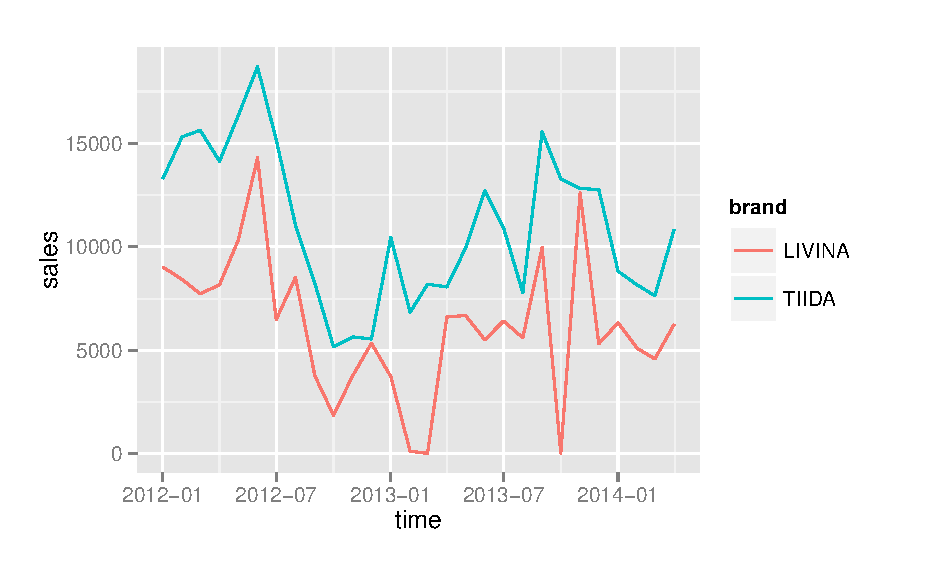
\includegraphics[width=13cm]{sales_LIVINA.eps}
\caption{骊威、骐达月销售量}
\label{fig:骊威、骐达销售数据}
\end{figure}

图\ref{fig:骊威、骐达销售数据}显示,两种车型的销量可能存在较强的正相关。我们通过散点图和线性拟合来进一步观察,如图\ref{fig:骊威、骐达散点图}所示。

\begin{figure}[htb]
\centering
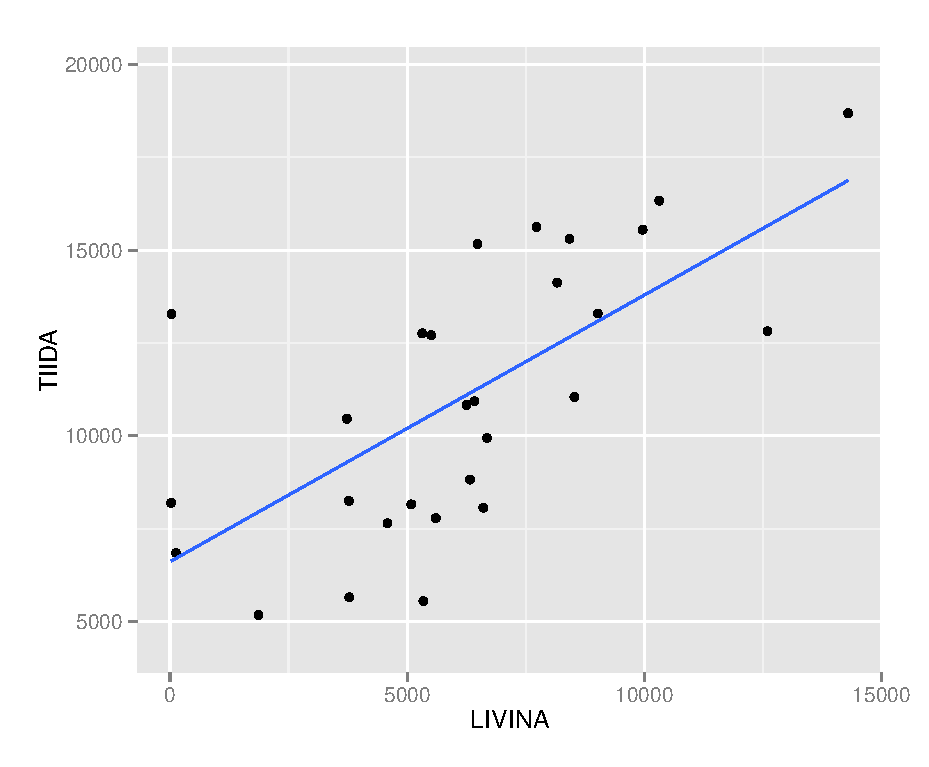
\includegraphics[width=11cm]{LIVINA_smooth.eps}
\caption{骊威、骐达销量散点图}
\label{fig:骊威、骐达散点图}
\end{figure}

图\ref{fig:骊威、骐达散点图}中也显示了两种汽车销量的正相关性。经过计算,骊威和骐达两者销量的相关系数为$\rho=0.67$。

再选择另一组数据进行比较。英朗(EXCELLE)和英朗XT(EXCELLEXT)是上海通用别克的两个汽车品牌,他们也有很多相同型号的配件,如主控板、火花塞等。这两个品牌过去两年的销售数据如图\ref{fig:英朗销售数据}所示。

\begin{figure}[htb]
\centering
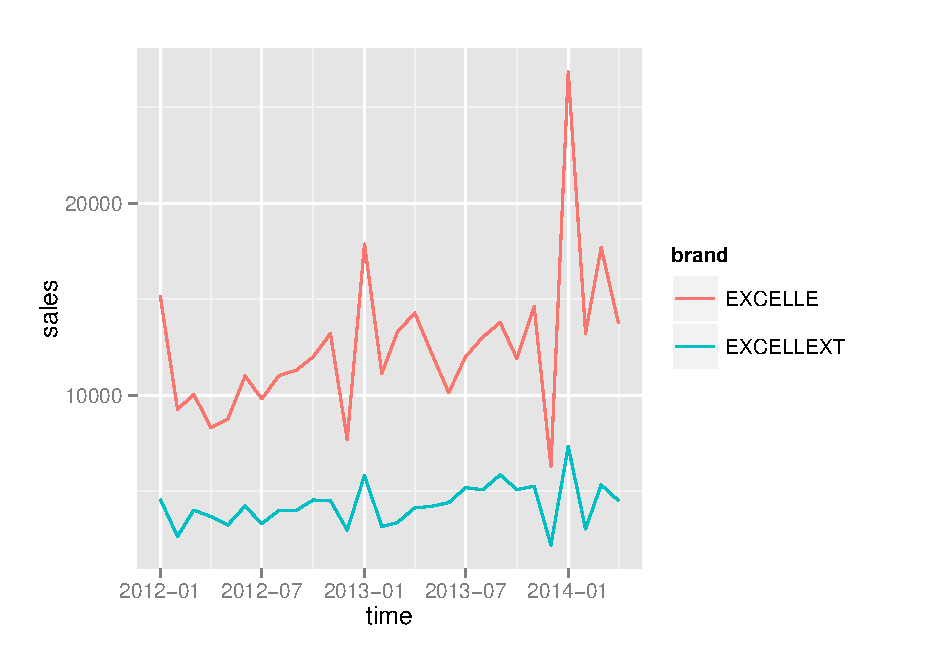
\includegraphics[width=13cm]{sales_EXCELLE.eps}
\caption{英朗、英朗XT月销售量}
\label{fig:英朗销售数据}
\end{figure}

图\ref{fig:英朗销售数据}中的两条曲线变化趋势基本相同,显示了比较强的正相关。相应的散点图和线性拟合如图\ref{fig:英朗散点图}所示。

\begin{figure}[htb]
\centering
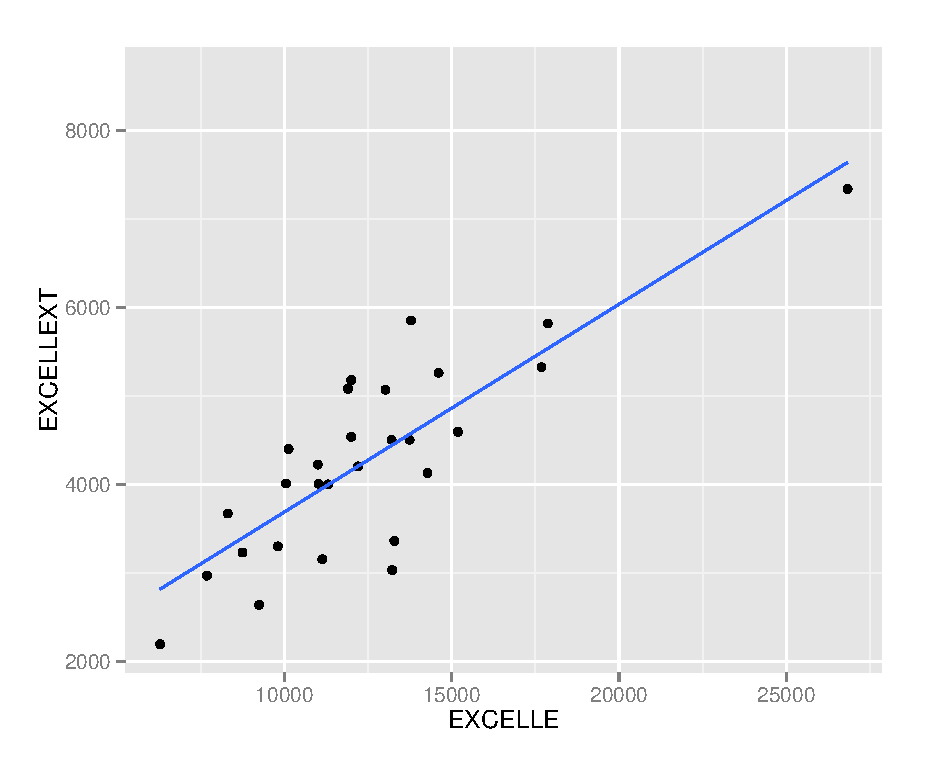
\includegraphics[width=11cm]{EXCELLE_smooth.eps}
\caption{英朗、英朗XT销量散点图}
\label{fig:英朗散点图}
\end{figure}

经过计算,英朗和英朗XT两者销量的相关系数为$\rho=0.82$。这两个品牌销量的相关性比骊威、骐达的相关性更强。同时,这两组数据说明,汽车行业中一些定位比较接近,有较多共同配件的汽车,它们的销量很可能是正相关的。

在本章的讨论中,我们已经知道,需求之间的正相关性会使得改进的效果减弱,改进前后的库存差别不明显。因此,对于汽车行业来说,是否要通过合并部件库存来降低总库存,是需要谨慎考虑,仔细论证的一件事情。
















